\documentclass{beamer}

\usecolortheme[RGB={205,173,0}]{structure}

\usepackage[spanish,es-noshorthands]{babel}
\usepackage{tikz}
\usetikzlibrary{calendar}

%\usepackage[spanish,activeacute,es-tabla]{babel}
\usepackage[utf8]{inputenc} % mac utf8
\usepackage{beamerthemesplit}


\usepackage{graphicx}
\DeclareGraphicsExtensions{.png,.pdf,.jpg}

\usefonttheme{professionalfonts} % fuentes de LaTeX 
\usetheme{Dresden}	% tema escogido en este ejemplo 

%\usetheme{Boadilla}
\usepackage{minted}
\usepackage{ucs}

\newtheorem{Teorema}{Teorema} 
\newtheorem{Ejemplo}{Ejemplo} 
\newtheorem{Definicion}{Definici\’on} 
\newtheorem{Corolario}{Corolario} 
\newtheorem{Prueba}{Prueba}
\newtheorem{practica} [Corolario]{Práctica} 
\newtheorem{teorema} [Teorema] {Teorema}
\newtheorem{ejemplo} [Ejemplo] {Ejemplo}
\newtheorem{definicion} [Definicion]{Definición} 
\newtheorem{ejercicio} [Corolario]{Ejercicio} 
\newtheorem{lema} [theorem] {Lema}

\setbeamertemplate{theorems}[numbered] 
\setbeamertemplate{caption}[numbered]


\usebackgroundtemplate{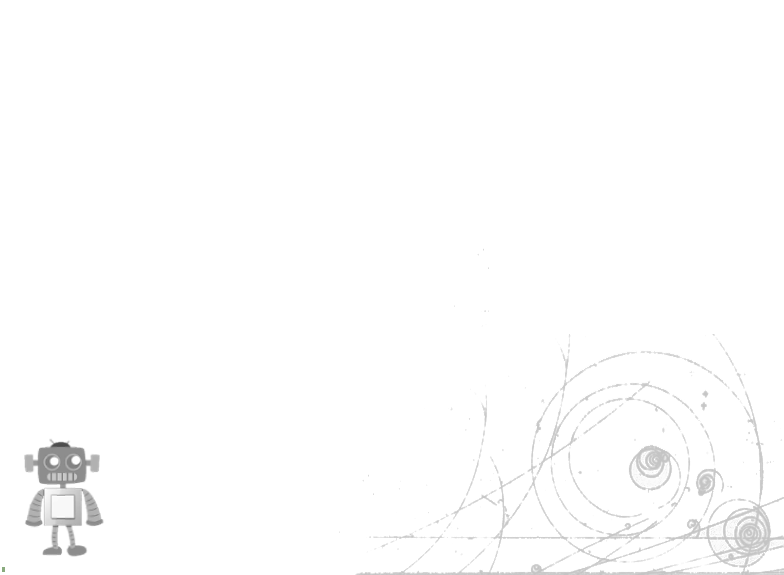
\includegraphics[width=\paperwidth,height=\paperheight]{./img/back.png}}

\title[]{Tema 2 - Introducción Sistemas Inteligentes}
\author[José A Montenegro (jmmontes@uma.es)]{José A. Montenegro}
\institute{Dpto. Lenguajes y Ciencias de la Computación\\
ETSI Informática. Universidad de Málaga\\
jmmontes@uma.es}
\date{\today}

%###########################################################################
% FootLine
%###########################################################################

\setbeamertemplate{footline} {%
\leavevmode%
  \hbox{\begin{beamercolorbox}[wd=.5\paperwidth,ht=2.5ex,dp=1.125ex,leftskip=.3cm plus1fill,rightskip=.3cm]{author in head/foot}%
    \usebeamerfont{author in head/foot}\insertshortauthor 
  \end{beamercolorbox}%
  
  \begin{beamercolorbox}[wd=.5\paperwidth,ht=2.5ex,dp=1.125ex,leftskip=.3cm,rightskip=.3cm plus1fil]{title in head/foot}%
    Sistemas Inteligentes\hfill    \insertpagenumber /\insertdocumentendpage
  \end{beamercolorbox}}%
  \vskip0pt%
}%

%###########################################################################
% Document
%###########################################################################

\begin{document}

%\setbeamertemplate{headline}[title slide]
%\setbeamertemplate{footline}[title slide]


%###########################################################################
% Título
%###########################################################################
\begin{frame}

\includegraphics[height=0.1\textheight]{./img/logoUma.png} \hspace*{3cm}

\includegraphics[height=0.1\textheight]{./img/logoInf.png}   \hspace*{3.5cm}

\includegraphics[height=0.1\textheight]{./img/logoLcc.png}  

\titlepage


\setbeamertemplate{footline}[body]
\setbeamertemplate{headline}[body]
\end{frame}

%###########################################################################
% Contenidos
%###########################################################################
\small
\section[Resumen]{}
\frame{\tableofcontents}

%%%%%%%%%%%%%%%%%%%%%%%%%%%%%%%%
%%%%%%%%%%%%%%%%%%%%%%%%%%%%%%%%
%SECCION %%%%%%%%%%%%%%%%%%%%%%%%%%%%%%%
%%%%%%%%%%%%%%%%%%%%%%%%%%%%%%%%
%%%%%%%%%%%%%%%%%%%%%% 

%%%%%%%%%%%%%%%%%%%%%%%%%%%%%%%%
%%%%%%%%%%%%%%%%%%%%%%%%%%%%%%%%
%\begin{frame}  \small \begin{ejercicio} \end{ejercicio} \pause \textit{\underline{Solución}}:\\ \end{frame} 
%%%%%%%%%%%%%%%%%%%%%%%%%%%%%%%%
%%%%%%%%%%%%%%%%%%%%%%%%%%%%%%%%
%EJERCICIO %%%%%%%%%%%%%%%%%%%%%%%%%%%%%%%
%%%%%%%%%%%%%%%%%%%%%%%%%%%%%%%%



\section{¿Qué es IA?}
%%%%%%%%%%%%%%%%%%%%%%%%%%%%%%%%
%%%%%%%%%%%%%%%%%%%%%%%%%%%%%%%%
\begin{frame} [fragile] \frametitle{Programación ``Tradicional''} \footnotesize


\begin{minted}[frame=lines,framesep=2mm,baselinestretch=1.2,bgcolor=white,fontsize=\scriptsize,linenos]
{java}
class IfElseDemo { 

public int  Calcula (int testscore , int n_assig, int …) { 
	 int grade=0;

	if (testscore >= 90 & n_assig >=5 )  { grade = ‘10'; } 
	else if (testscore >= 80 & n_assig >=3 ) { grade = ‘9'; } 
	else  if (testscore >= 70 & n_assig >=1) { grade = ‘7'; } 
	else  if (testscore >= 60) { grade = ‘6'; } 
	else { grade = ‘4'; }
	}
	return grade;
}

\end{minted}

\end{frame} 

%%%%%%%%%%%%%%%%%%%%%%%%%%%%%%%%
%%%%%%%%%%%%%%%%%%%%%%%%%%%%%%%%

\begin{frame} \frametitle{¿Qué es IA?} \footnotesize


\begin{figure}
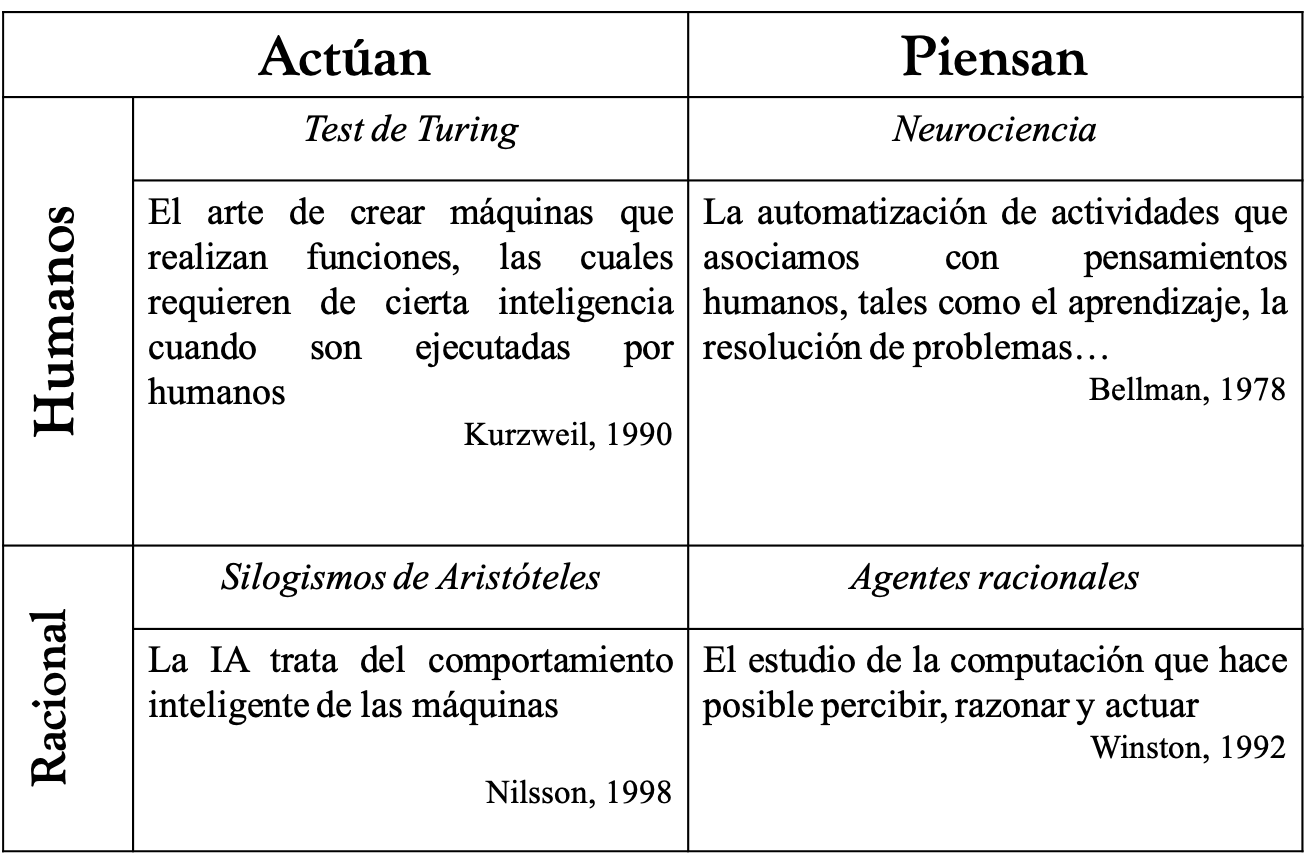
\includegraphics[scale=0.45]{./img/queEsIA}
\end{figure}

\end{frame} 

%%%%%%%%%%%%%%%%%%%%%%%%%%%%%%%%

\begin{frame} \frametitle{Historia y Futuro IA} \footnotesize


Responde a las siguientes preguntas:
\begin{itemize}
\item Aportaciones Alan Turing IA.
\item Lenguaje programación para IA. Establezca breve descripción 
\item ¿Qué es deep blue? 
\item Tensorflow
\item Procesamiento del lenguaje mediante IA
\item ¿Cómo funciona Google driverless car (Waymo)?
\item ¿Cómo funciona Asistentes: Siri, Hound, AlexaWiki?
\item ¿Qué es WEKA?
\item Machine Learning
\item Deap Learning
\item IA en Videojuegos
\end{itemize}
\end{frame} 


\section{Paradigmas y tendencias en la investigación de la IA}
%%%%%%%%%%%%%%%%%%%%%%%%%%%%%%%%
%%%%%%%%%%%%%%%%%%%%%%%%%%%%%%%%
 \begin{frame}\frametitle{Paradigmas y tendencias en la investigación de la IA} \footnotesize  
 

\begin{itemize}
\item Modelo simbólico – Lógico: reglas de producción o semántico.
\item Modelo conexionista o emergente – Redes neuronales.
\item Modelo basado en datos (operativo) – Aprendizaje profundo.
\item Modelo colectivo – Inteligencia colectiva
\item Modelo evolutivo – Algoritmo genético.
\item Modelo corpóreo – Agentes inteligentes (agentes reactivos).
\end{itemize}

%%https://cibernetica.wordpress.com/2021/05/13/modelos-de-la-inteligencia-artificial-el-conexionista/

%%https://cibernetica.wordpress.com/category/desarrollo-ia/
\end{frame}


\section{Agentes Inteligentes}
%%%%%%%%%%%%%%%%%%%%%%%%%%%%%%%%
%%%%%%%%%%%%%%%%%%%%%%%%%%%%%%%%


%%%%%%%%%%%%%%%%%%%%%

 \begin{frame}\frametitle{Agentes y entorno} \footnotesize  
 
\begin{center}
	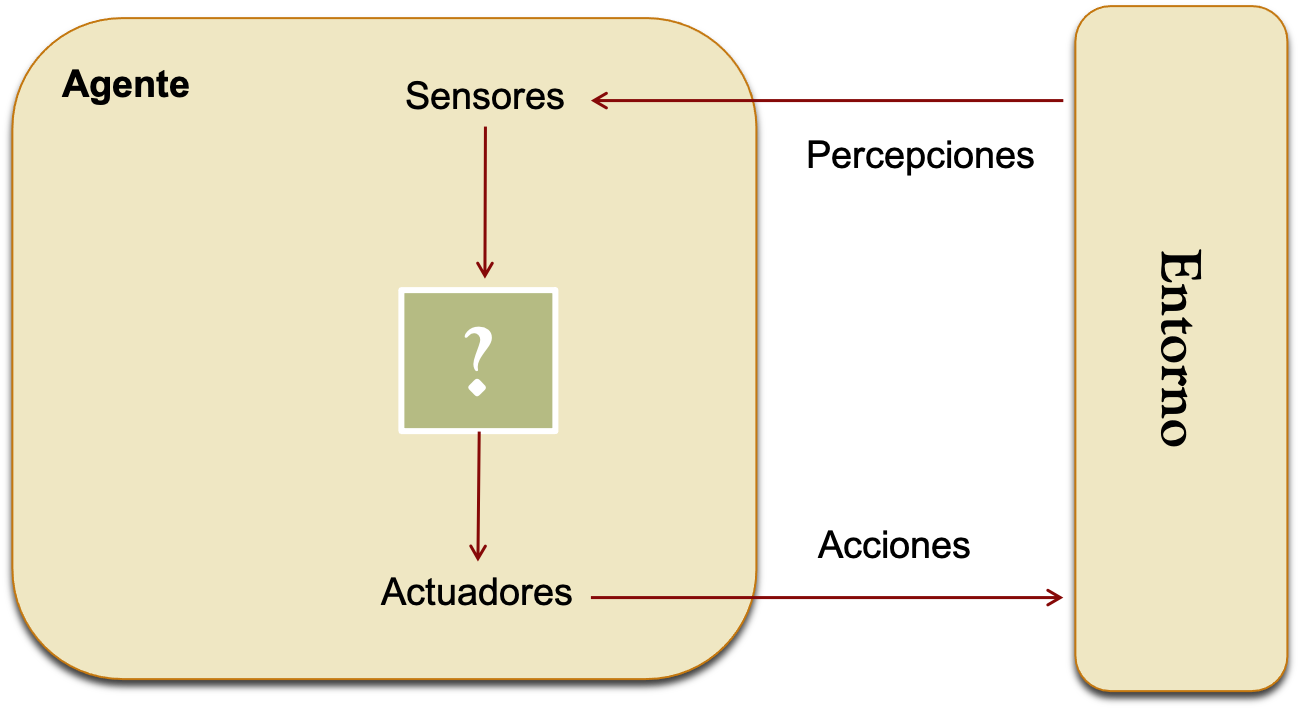
\includegraphics[scale=0.45]{img/AgenteyEntorno} 
\end{center}
\end{frame}


%%%%%%%%%%%%%%%%%%%%%

 \begin{frame}\frametitle{Agentes y entorno} \footnotesize  
 
\begin{center}
	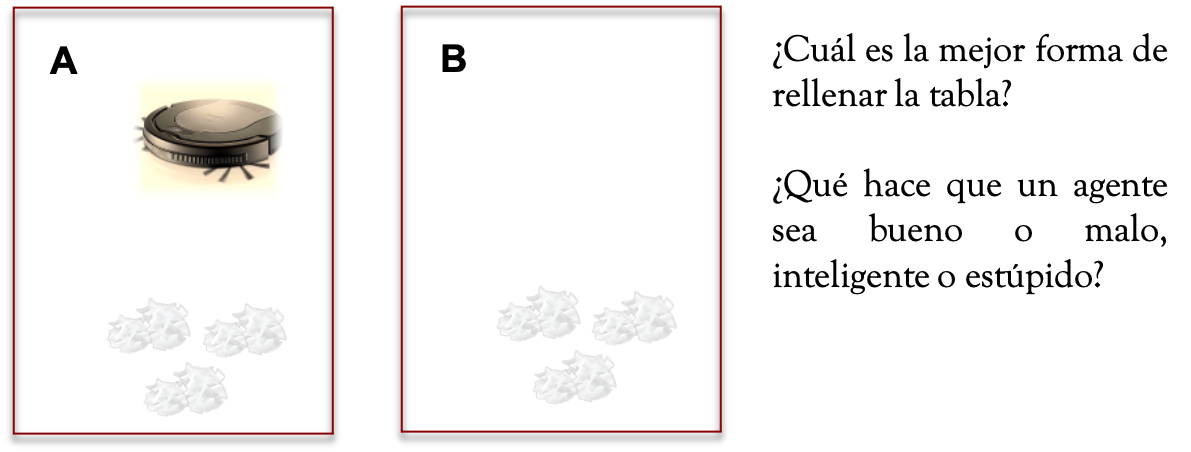
\includegraphics[scale=0.4]{img/aspiradora} \\
	
	\vspace*{0,8cm}
	\begin{tabular}{|c|c|}
	\hline 
		\textbf{Secuencia de percepciones} & \textbf{Acción} \\ 
	\hline 
	[A,Limpio] & Derecha\\
	\hline 
	[A,Sucio]  & Aspirar\\
	\hline 
	[B,Limpio] & Izquierda\\
	\hline 
	[B,Sucio] & Aspirar\\
	\hline 
	\end{tabular} 

	
\end{center}
\end{frame}

%%%%%%%%%%%%%%%%%%%%%%%%%%%%%%%%


\begin{frame}\frametitle{Ejemplo Agentes y entorno} \footnotesize  
 
\begin{center}
	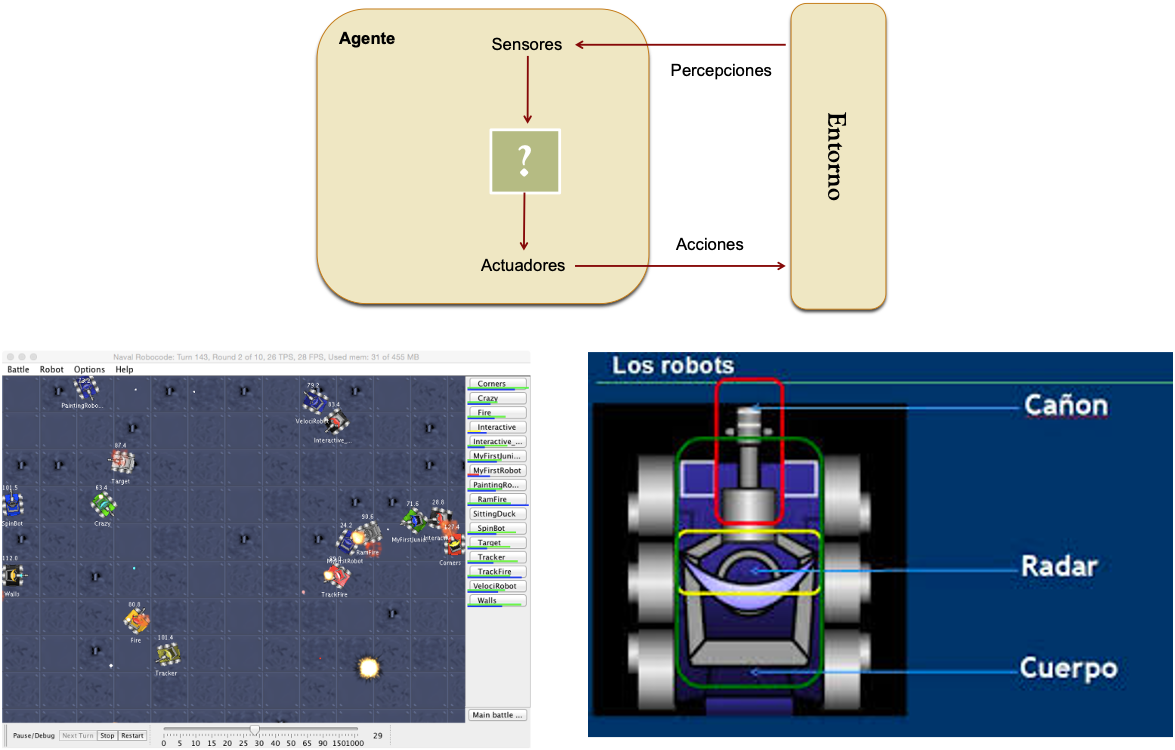
\includegraphics[scale=0.45]{img/agenteRobocode} 
\end{center}
\end{frame}

%%%%%%%%%%%%%%%%%%%%%%%%%%%%%%%%
\begin{frame}\frametitle{Medidas de Rendimiento} \footnotesize  
 
\begin{itemize}
\item Un agente racional es aquel que hace lo correcto, que se  traduce hasta ahora en rellenar correctamente la tabla.
\item Como primera aproximación hacer lo correcto es aquello que permite al agente obtener un resultado mejor.
\begin{itemize}
\item Necesitamos una manera de medir el éxito.
\item Por ejemplo, un punto por cada cuadrícula limpia en cada período de tiempo, penalizando la luz y el ruido.
\end{itemize}
\item En general, la elección de una medida de rendimiento no es una tarea fácil.

\end{itemize}

\end{frame}

%%%%%%%%%%%%%%%%%%%%%%%%%%%%%%%%
\begin{frame}\frametitle{Agente Racional} \footnotesize  
 
 
 Racionalidad depende de cuatro factores:

\begin{enumerate}
 \item  La medida de rendimiento que define el criterio de éxito 
  \item  El conocimiento acumulado del medio en el que habita el agente 
  \item  Las acciones que puede llevar a cabo
  \item  La secuencias de percepciones del agente hasta ese momento.

 \end{enumerate} 
 
 \vspace*{0,8cm}
 \begin{block}{Definición: Agente Racional}
En cada posible secuencia de percepciones, un agente racional deberá emprender aquella acción que supuestamente maximice su medida de rendimiento, basándose en las evidencias aportadas por la secuencia de percepciones y en el conocimiento que el agente tiene almacenado.
\end{block}

\end{frame}

\section{Naturaleza del Entorno}
%%%%%%%%%%%%%%%%%%%%%%%%%%%%%%%%
%%%%%%%%%%%%%%%%%%%%%%%%%%%%%%%%
\begin{frame}\frametitle{Entorno Trabajo} \footnotesize  
 
 El entorno de trabajo de un agente lo forman:

\begin{enumerate}
 \item  Medidas de rendimiento
  \item  Entorno
  \item  Actuadores
  \item  Sensores

 \end{enumerate} 
 
 \vspace*{0,4cm}
\begin{center}
	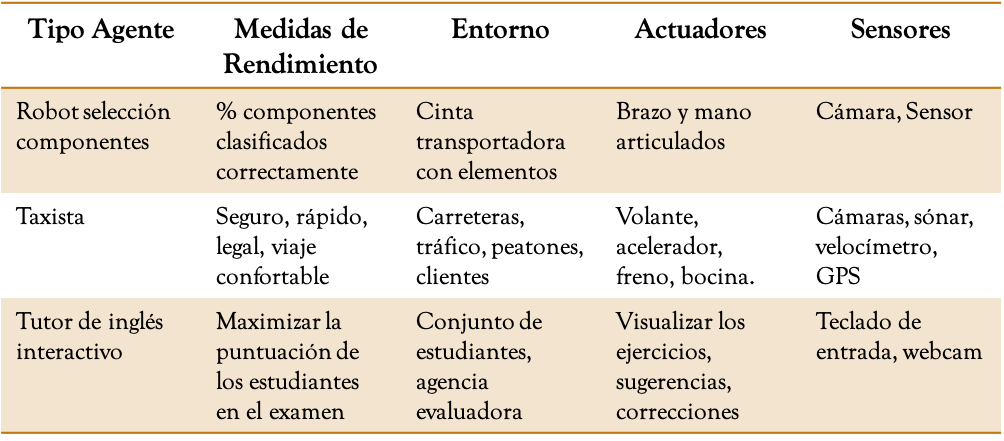
\includegraphics[scale=0.45]{img/EntornoTrabajoTabla} 
\end{center}

\end{frame}

%%%%%%%%%%%%%%%%%%%%%%%%%%%%%%%%
\begin{frame}\frametitle{Propiedades de Entornos Trabajo} \footnotesize  
 
\begin{itemize}
\item \textbf{Totalmente Observable} vs.  \textbf{Parcialmente Observable}\\
Si los sensores del agente proporciona acceso al estado completo del medio en cada momento, entonces se dice que el entorno de trabajo es totalmente observable. (No necesita mantener estado interno para saber que sucede)

\item \textbf{Determinista} vs.  \textbf{Estocástico}\\
Si el siguiente estado del medio está totalmente determinado por el estado actual y la acción ejecutada por el agente, entonces se dice que el entorno es determinista.

\item \textbf{Episódico} vs.  \textbf{Secuencial}\\
En un entorno de trabajo episódico, la experiencia del agente se divide en episodios atómicos. Cada episodio consiste en la percepción del agente y la realización de una única acción posterior.

\end{itemize}


\end{frame}
%%%%%%%%%%%%%%%%%%%%%%%%%%%%%%%%
\begin{frame}\frametitle{Propiedades de Entornos Trabajo} \footnotesize  
 
\begin{itemize}
\item \textbf{Estático} vs.  \textbf{Dinámico}\\
Si el entorno puede cambiar cuando el agente está deliberando, entonces se dice que el entorno es dinámico para el agente.

\item \textbf{Discreto} vs.  \textbf{Continuo}\\
Se aplica al estado del medio, a la forma que se maneja el tiempo y a las percepciones y acciones del agente. (Ajedrez vs taxi)


\item \textbf{Agente Individual} vs.  \textbf{Multiagente}\\
Dentro del multiagente tenemos competitivo y cooperativo.
\end{itemize}

 \vspace*{0,4cm}

Caso más complejo es parcialmente observable, estocástico, secuencial, dinámico, continuo y multiagente. 
\end{frame}



\section{Estructura de los Agentes}
%%%%%%%%%%%%%%%%%%%%%%%%%%%%%%%%
%%%%%%%%%%%%%%%%%%%%%%%%%%%%%%%%
\begin{frame}\frametitle{Estructura de los Agentes} \footnotesize  
 
 
 Previamente se describe los agentes por su conducta. 
Acción como resultado de una secuencia de percepciones.


\begin{center}
\textit{Trabajo de la IA es diseñar el programa del agente.}\\
Agente = arquitectura + programa
\end{center}

Veremos a continuación cuatro tipos básicos de programas:

\begin{itemize}
\item Agentes reactivos simples
\item Agentes reactivos basados en modelos
\item Agentes basados en objetivos
\item Agentes basados en utilidad
\end{itemize}

\end{frame}


%%%%%%%%%%%%%%%%%%%%%%%%%%%%%%%%
\begin{frame}\frametitle{Programa de los Agentes} \footnotesize  
 
Generalmente reciben las percepciones como entrada de los sensores y devuelven una acción a los actuadores. 

 \vspace*{0,1cm}
 
 El \textbf{desafío} clave de la IA es encontrar la forma de escribir programas, que reproduzcan un comportamiento racional a partir de una \textbf{pequeña cantidad de código} en vez de partir de una tabla con un gran número de entradas.

\begin{center}
	
\includegraphics[scale=0.4]{img/ProgramaAgentes} 
\end{center}


\end{frame}

%%%%%%%%%%%%%%%%%%%%%%%%%%%%%%%%
\begin{frame}\frametitle{Agentes Reactivos Simples} \footnotesize  
 
 \begin{itemize}
 \item Es el tipo de agente más sencillo.
 \item Seleccionan las acciones sobre la base de las percepciones actuales, ignorando el resto de las percepciones históricas.
 \item Regla condición- acción: si acción entonces condición.
 \end{itemize}
 
 \begin{center}
	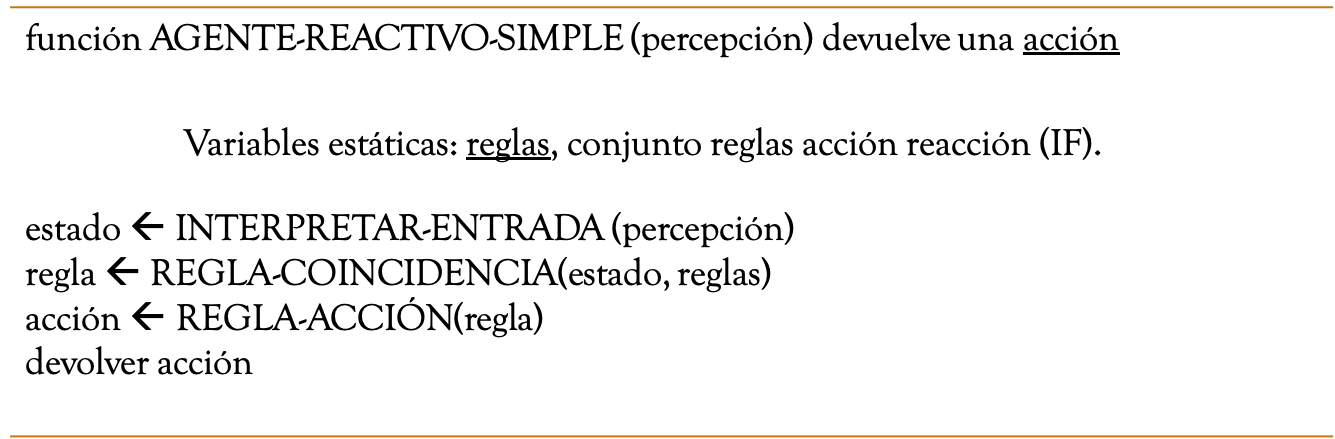
\includegraphics[scale=0.4]{img/AgentesReactivosSimples} 
\end{center}

\end{frame}
%%%%%%%%%%%%%%%%%%%%%%%%%%%%%%%%
\begin{frame}\frametitle{Agentes Reactivos Simples} \footnotesize  
 
 \begin{center}
	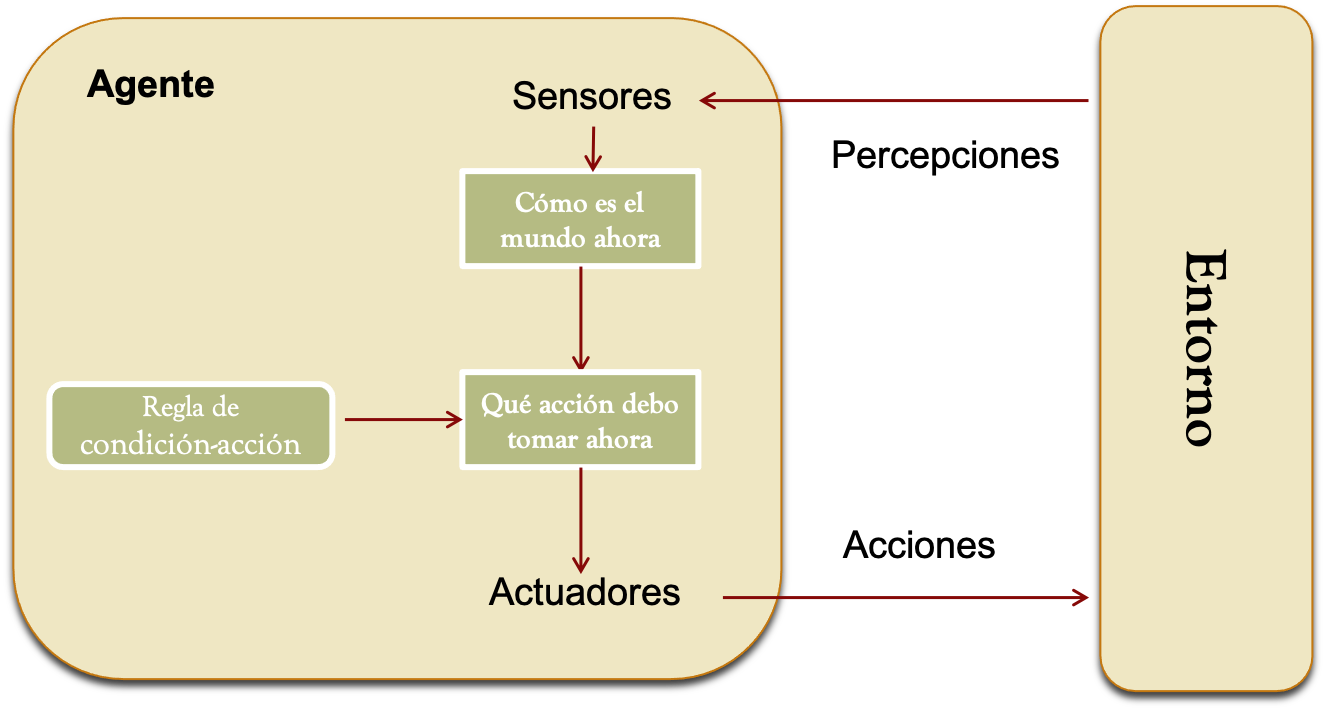
\includegraphics[scale=0.4]{img/AgentesReactivosSimplesDibujo} 
\end{center}

\end{frame}
%%%%%%%%%%%%%%%%%%%%%%%%%%%%%%%%
\begin{frame}\frametitle{Agentes Reactivos basado en Modelos} \footnotesize  
 
 \begin{itemize}
 \item Para manejar la visibilidad parcial, los agentes almacenan información de las partes del mundo que no pueden ver.
 \item Agente mantiene un estado interno.
 \item El conocimiento de cómo funciona el mundo se denomina modelo del mundo
 \end{itemize}
 
 \begin{center}
	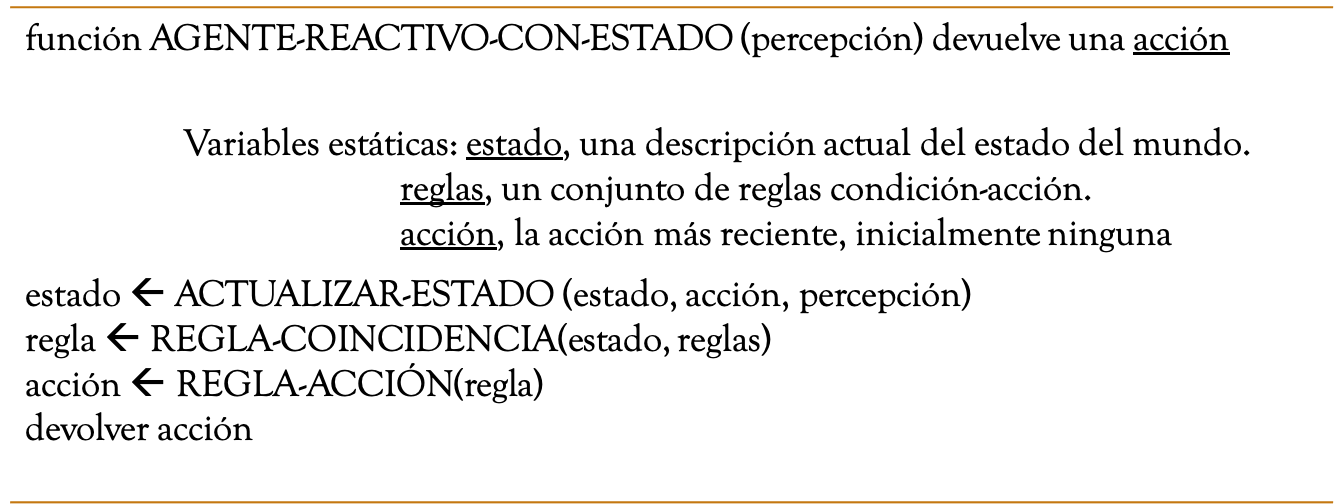
\includegraphics[scale=0.4]{img/AgentesReactivosModelos} 
\end{center}

\end{frame}
%%%%%%%%%%%%%%%%%%%%%%%%%%%%%%%%
\begin{frame}\frametitle{Agentes Reactivos basado en Modelos} \footnotesize  
 
 \begin{center}
	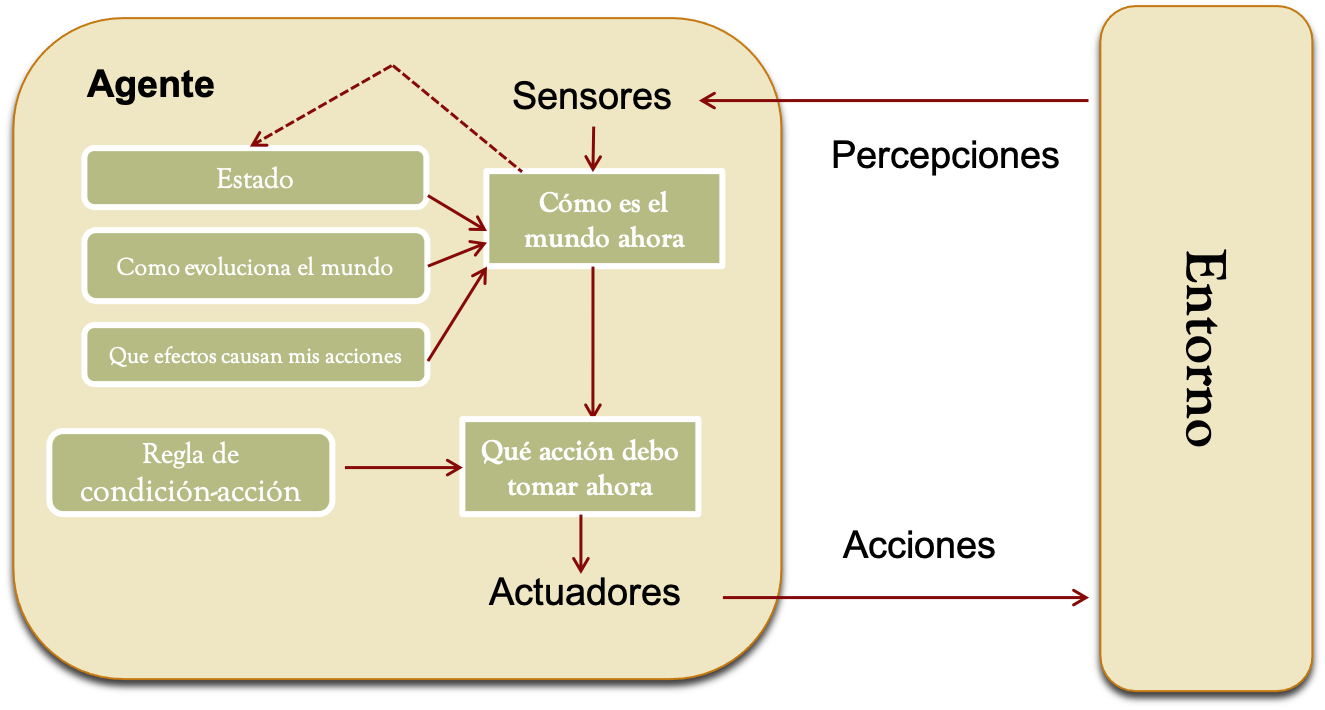
\includegraphics[scale=0.4]{img/AgentesReactivosModelosDibujo} 
\end{center}

\end{frame}

%%%%%%%%%%%%%%%%%%%%%%%%%%%%%%%%
\begin{frame}\frametitle{Agentes basados en objetivos} \footnotesize  
 
 \begin{itemize}
 \item  El conocimiento sobre el estado actual del mundo no siempre es suficiente para predecir que hacer.
 \item Es necesario algún tipo de información sobre su meta.
 \end{itemize}

 \begin{center}
	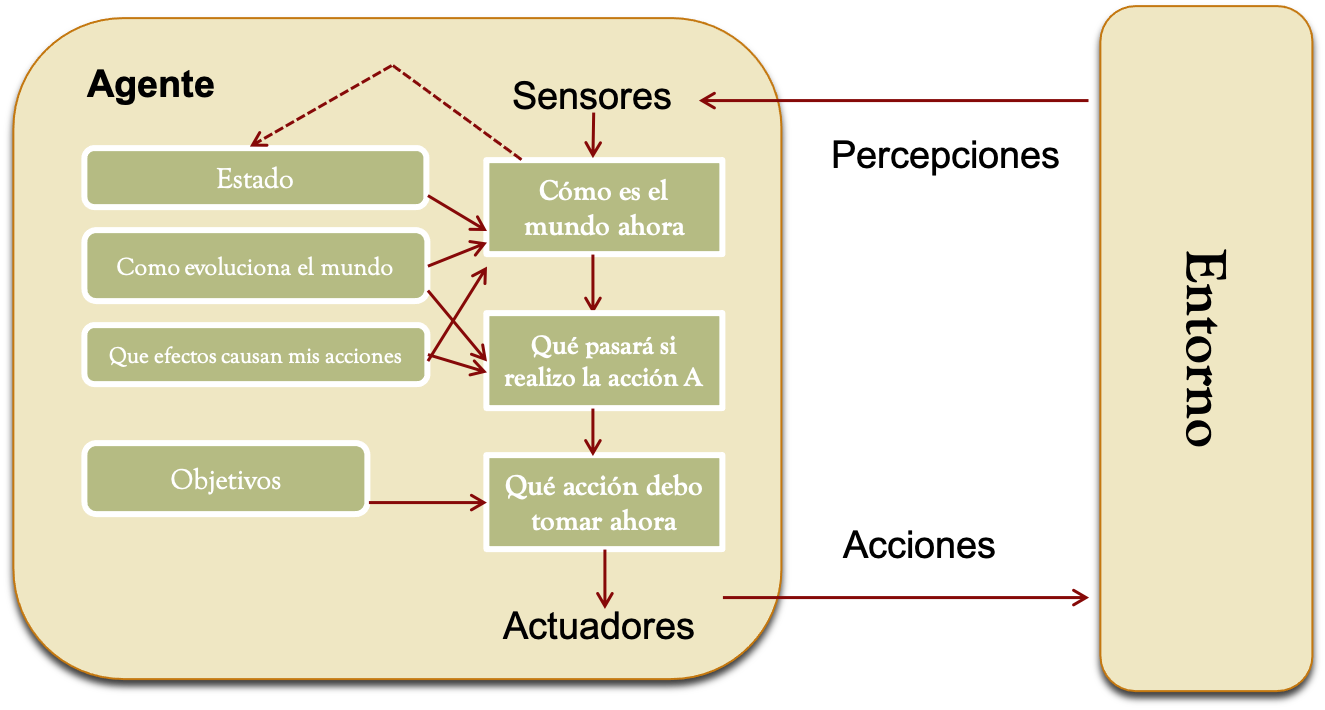
\includegraphics[scale=0.4]{img/AgentesBasadosObjetivos} 
\end{center}

\end{frame}

%%%%%%%%%%%%%%%%%%%%%%%%%%%%%%%%
\begin{frame}\frametitle{Agentes basado en utilidad} \footnotesize  
 
 \begin{itemize}
 \item  Las metas producen un valor global. En ocasiones es necesario medir el valor de éxito de cada estado. 
 \item  Definimos una función de utilidad que proyecta un estado en un número real que representa el éxito. 
 \end{itemize} 
 


 \begin{center}
	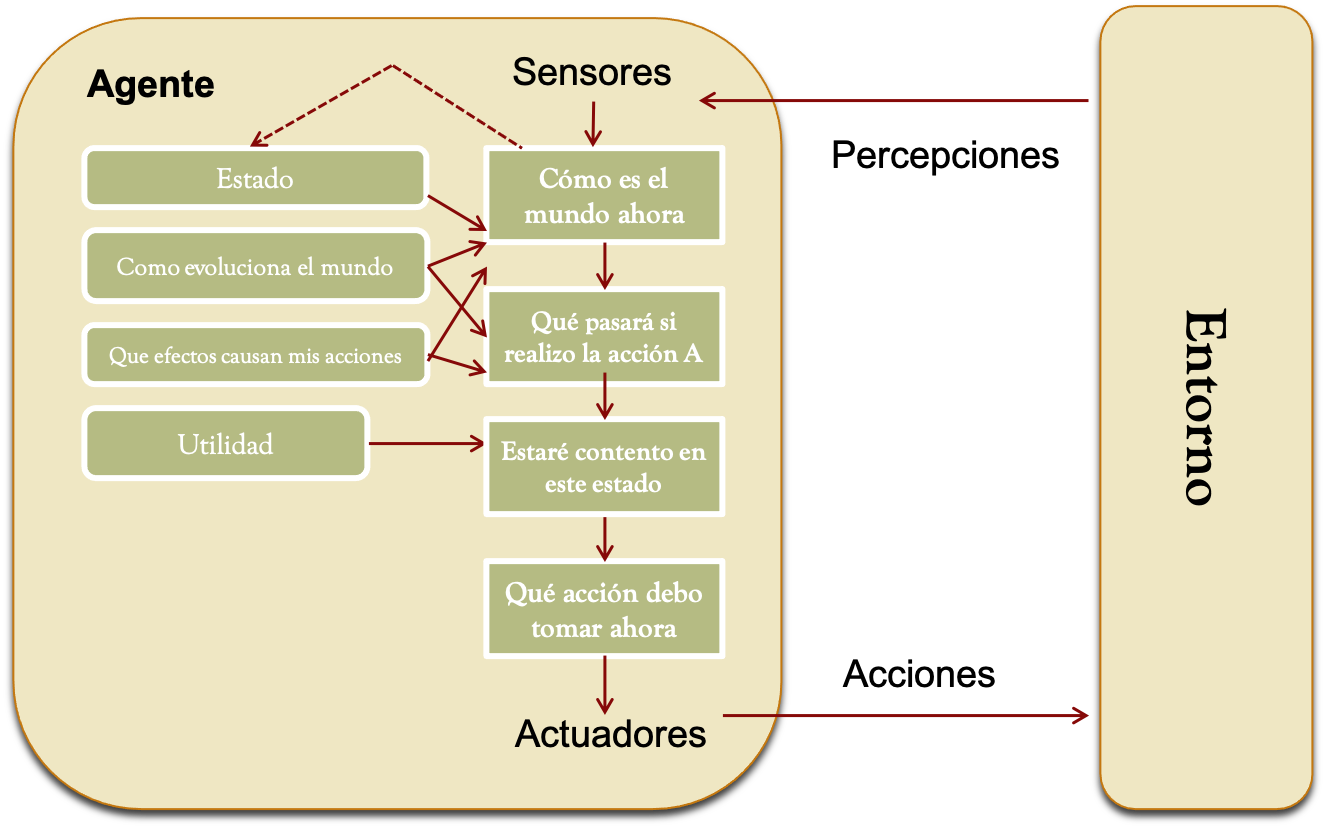
\includegraphics[scale=0.35]{img/AgentesBasadosUtilidad} 
\end{center}

\end{frame}

%%%%%%%%%%%%%%%%%%%%%%%%%%%%%%%%
\begin{frame}\frametitle{Agentes que aprenden} \footnotesize  
 
 
  \begin{itemize}
  \item  El aprendizaje permite que opere en medios inicialmente desconocidos y que sea más competente si sólo utilizase un conocimiento inicial.
  \item  Nivel de actuación $\rightarrow$ Recompensas o penalizaciones. 
 \end{itemize} 
 

 \begin{center}
	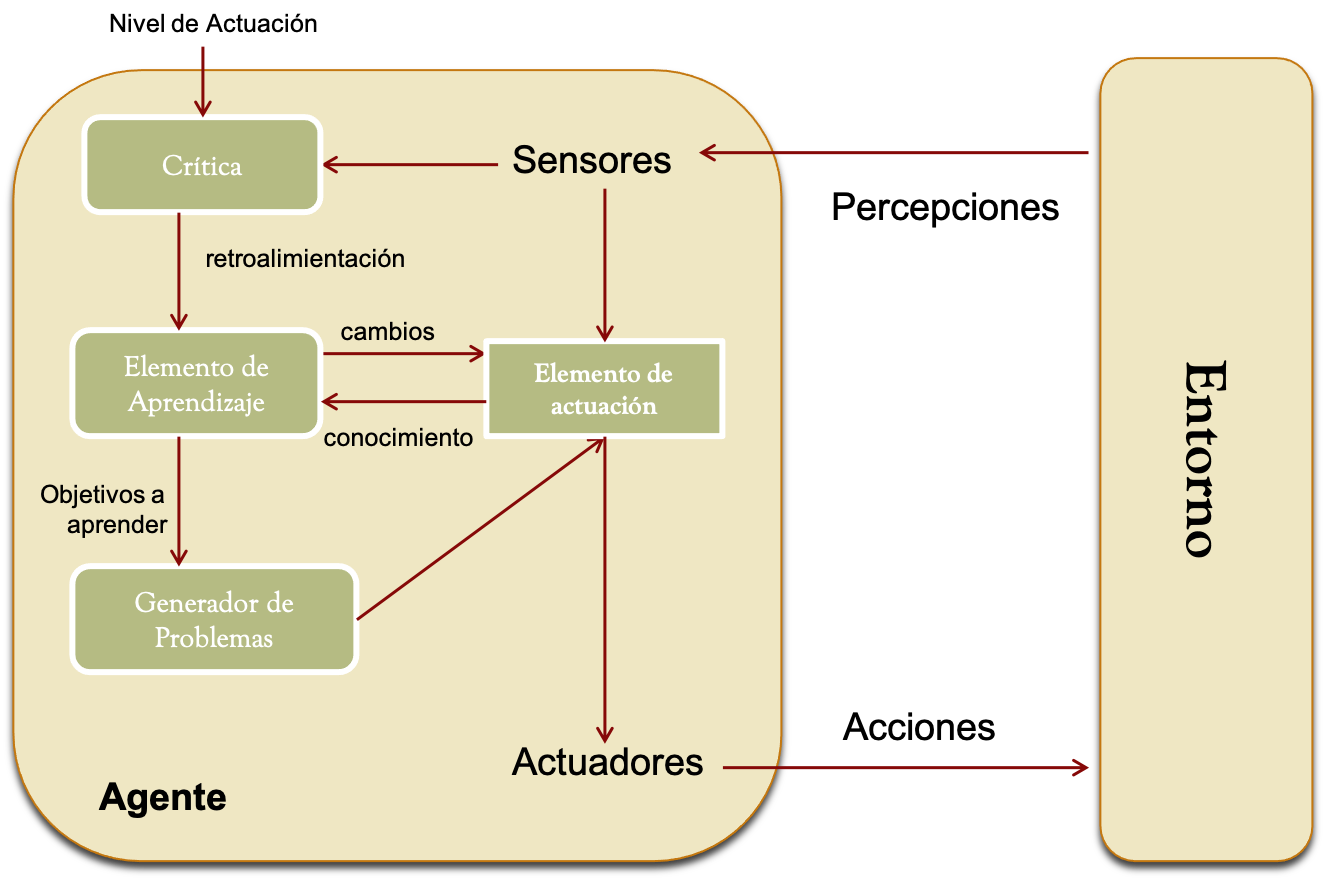
\includegraphics[scale=0.35]{img/AgentesAprenden} 
\end{center}

\end{frame}


 %%%%%%%%%%%%%%%%%%%%%%%%%%%%%%%%
%%%%%%%%%%%%%%%%%%%%%%%%%%%%%%%%
\section{ToDo: Espacios de estados}
%%%%%%%%%%%%%%%%%%%%%%%%%%%%%%%%
%%%%%%%%%%%%%%%%%%%%%%%%%%%%%%%%

%%%%%%%%%%%%%%%%%%%%%%%%%%%%%%%%
\begin{frame}  \small  

ToDo: \\

Concepto de representación simbólica\\
Espacios de estados

\end{frame} 


\section{Agentes resolventes-problemas}
%%%%%%%%%%%%%%%%%%%%%%%%%%%%%%%%
%%%%%%%%%%%%%%%%%%%%%%%%%%%%%%%%

\begin{frame} \frametitle{Agentes resolventes-problemas} \footnotesize

\begin{itemize}
\item Agentes inteligentes deben maximizar su rendimiento.

\begin{itemize}
\item Elegir objetivo y satisfacerlo, implica formulación objetivo
\item Formulación problema, dado un objetivo, es el proceso de decidir acciones y estados a considerar.
\end{itemize}


\item Agente con distintas opciones inmediatas de valores desconocidos puede decidir qué hacer, examinando las diferentes secuencias posibles de acciones que le conduzcan a estados de valores conocidos y entonces escoger la mejor secuencia.


\item Búsqueda es el proceso de hallar la secuencia.

\begin{itemize}
\item Algoritmo de búsqueda toma como entrada un problema y devuelve una solución (secuencia de acciones).
\end{itemize}

\end{itemize}

\end{frame} 

%%%%%%%%%%%%%%%%%%%%%%%%%%%%%%%%

\begin{frame} \frametitle{Definición problema} \footnotesize

\begin{itemize}
\item Problema puede definirse con 4 componentes:

\begin{enumerate}
\item \textbf{Estado inicial}, donde comienza agente.
\item \textbf{Acciones} disponibles por el agente, p.ej. Función sucesor.
\item \textbf{Test objetivo}, determina si un estado es objetivo. 
\item \textbf{Costo camino},  asigna un costo numérico a cada camino.
\end{enumerate}


\end{itemize}

\begin{description}
\item[Espacio de estados]: Todos los estados alcanzables desde el estado inicial. Definido por el estado inicial y la función sucesor.
\item[Camino] : Secuencia estados conectados por una secuencia de acciones.
\item[Solución] : Camino estado inicial a un estado objetivo.
\begin{itemize}
\item \textbf{Calidad solución} viene dada por el costo del camino.
\item \textbf{Solución Óptima} coste mínimo de todas las soluciones.
\end{itemize}

\end{description}


\end{frame} 

%%%%%%%%%%%%%%%%%%%%%%%%%%%%%%%%

\begin{frame} \frametitle{Ejemplo problema} \footnotesize

\begin{center}
\textbf{Mundo Aspiradora}
\end{center}

\begin{description}
\item[Estados]: Dos localizaciones posibles y cada una puede estar sucia o no  $\rightarrow 2x 2^{2}=8$.
\item[Estado inicial]: Cualquier estado.
\item[Función sucesor]: Tres acciones posibles (Izquierda, Derecha, Aspirar)
\item[Test objetivo]: Todos los estados cuadrados limpios. 
\item[Costo camino]: Costo individual es 1, costo camino número pasos que lo componen.
\end{description}

\begin{figure}
\includegraphics[scale=0.45]{./img/Aspiradora}
\end{figure}

\end{frame} 

%%%%%%%%%%%%%%%%%%%%%%%%%%%%%%%%

\begin{frame} \frametitle{Ejemplo problema} \footnotesize


\begin{figure}
\includegraphics[scale=0.5]{./img/Aspiradora}
\end{figure}

\end{frame} 

%%%%%%%%%%%%%%%%%%%%%%%%%%%%%%%%

\begin{frame} \frametitle{Otro problema} \footnotesize


\begin{center}
\textbf{8-puzzle}
\end{center}

\begin{description}
\item[Estados]: Localización de las 8 fichas y el blanco.
\item[Estado inicial]: Cualquier estado.
\item[Función sucesor]: Cuatro acciones posibles (Izquierda, Derecha, Arriba, Abajo).
\item[Test objetivo]: Estado coincide con la configuración objetivo.
\item[Costo camino]: Costo individual es 1, costo camino número pasos que lo componen.
\end{description}

\begin{figure}
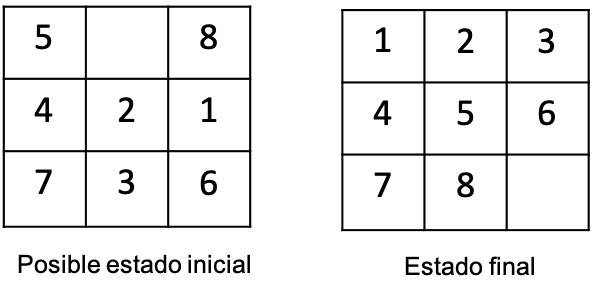
\includegraphics[scale=0.45]{./img/Puzzle8}
\end{figure}

\end{frame} 
\section{Búsqueda de Soluciones}
%%%%%%%%%%%%%%%%%%%%%%%%%%%%%%%%
%%%%%%%%%%%%%%%%%%%%%%%%%%%%%%%%
%%%%%%%%%%%%%%%%%%%%%%%%%%%%%%%%

\begin{frame} \frametitle{Resolución problema} \footnotesize

\begin{itemize}
\item  Normalmente el espacio de estados generado por el estado inicial y la función sucesor es representado por un \textbf{árbol de búsqueda}.
\item  Cuando un estado es alcanzable por varios caminos tendremos un \textbf{grafo de búsqueda}. 
\end{itemize}


\begin{figure}
\includegraphics[scale=0.45]{./img/nodoArbol}
\end{figure}

\end{frame} 

%%%%%%%%%%%%%%%%%%%%%%%%%%%%%%%%

\begin{frame} \frametitle{Resolución problema} \footnotesize

\begin{itemize}
\item  El algoritmo general sería comenzando en la raíz, escoge, comprueba y expande hasta que encuentra una solución o no existen más estados para expandir.
\end{itemize}


\begin{figure}
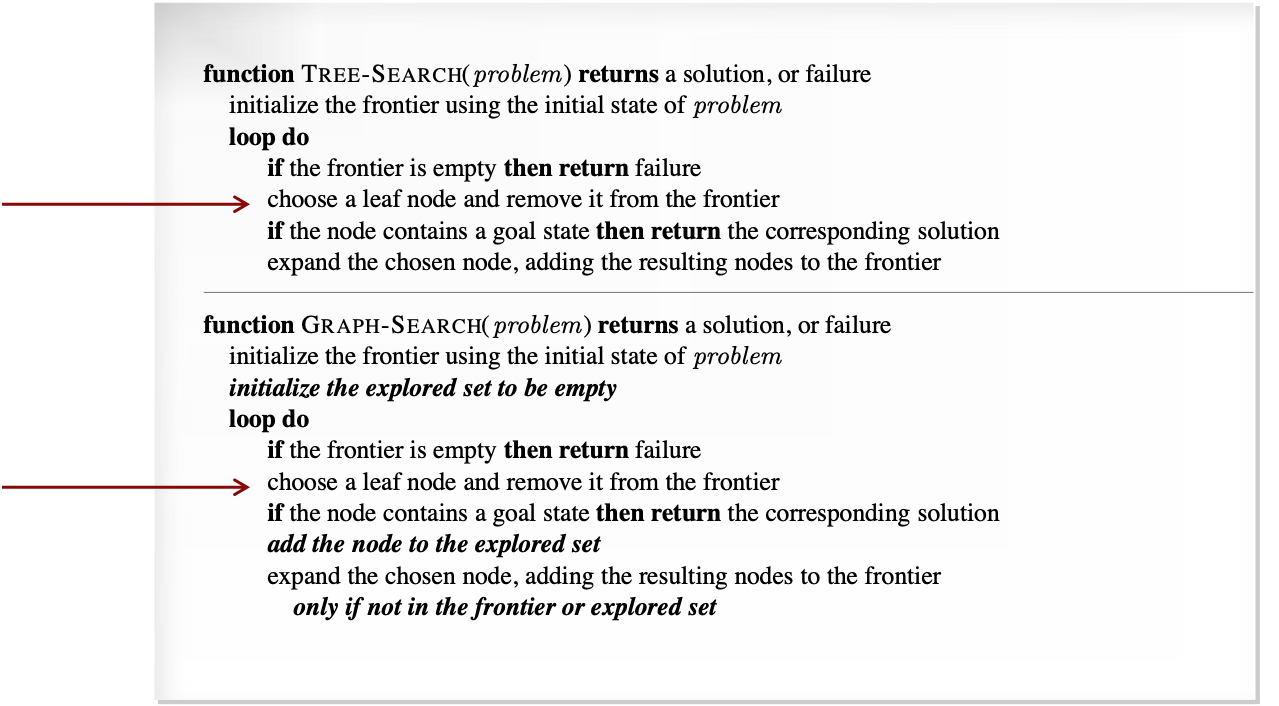
\includegraphics[scale=0.45]{./img/Arbol-Grafo}
\end{figure}

\end{frame} 

%%%%%%%%%%%%%%%%%%%%%%%%%%%%%%%%

\begin{frame} \frametitle{Resolución problema} \footnotesize

\begin{description}
\item [Frontera]: La colección (conjunto) de nodos (nodos hoja) que se generan pero no se ha expandido. 
\begin{itemize}
\item La estrategia de búsqueda será una función que seleccione del conjunto el siguiente nodo a expandir.
\end{itemize}
\end{description}


\begin{figure}
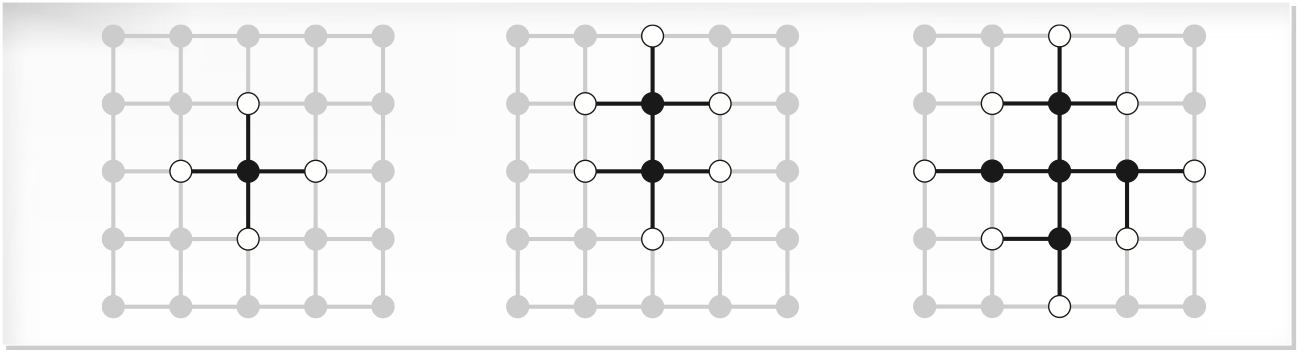
\includegraphics[scale=0.45]{./img/Frontera}
\end{figure}

\end{frame} 
%%%%%%%%%%%%%%%%%%%%%%%%%%%%%%%%

\begin{frame} \frametitle{Rendimiento de la resolución} \footnotesize

\begin{description}
\item [Completitud]: Garantizado algoritmo encuentra solución cuando existe.
\item [Optimización]: Encuentra la estrategia la solución óptima.
\item [Complejidad en tiempo]: Cuanto tarda en encontrar la solución.
\item [Complejidad en espacio]: Cuanta memoria necesita para el funcionamiento de la búsqueda.

\item [Eficiencia]: 
	\begin{itemize}
		\item Coste de la búsqueda, complejidad en tiempo y también uso memoria. 
		\item Coste total, coste de la búsqueda y coste del camino solución encontrado.
		\end{itemize}
\end{description}


\end{frame} 

%%%%%%%%%%%%%%%%%%%%%%%%%%%%%%%%
%%%%%%%%%%%%%%%%%%%%%%%%%%%%%%%%


%%%%%%%%%%%%%%%%%%%%%%%%%%%%%%%%
%\begin{frame}  \small  
%\end{frame} 


%%%%%%%%%%%%%%%%%%%%%%%%%%%%%%%%
%\begin{frame}  \small  
%\end{frame} 


%%%%%%%%%%%%%%%%%%%%%%%%%%%%%%%%
%\begin{frame}  \small  
%\end{frame} 


\begin{frame} %\frametitle{Preguntas}

%\begin{center}
%¡Gracias por su atención!\\
%\end{center}
\vspace*{2cm}

\begin{center}
\textbf{José A. Montenegro Montes} \\

\textit{Dpto. Lenguajes y Ciencias de la Computación}\\
\textit{ETSI  Informática. Universidad de Málaga}\\
\textbf{jmmontes@uma.es}
\end{center}

\vspace*{1,3cm}

 \hspace*{1.cm}
\includegraphics[height=0.1\textheight]{./img/logoUma.png} \hspace*{2.5cm}

\includegraphics[height=0.1\textheight]{./img/logoInf.png}   \hspace*{2.5cm}

\includegraphics[height=0.1\textheight]{./img/logoLcc.png}  


\end{frame} 

\end{document} 
